\documentclass{article}
\usepackage{pgf}
\usepackage{pgfpages}

% Options for packages loaded elsewhere
\PassOptionsToPackage{unicode}{hyperref}
\PassOptionsToPackage{hyphens}{url}
%

\usepackage{amsmath,amssymb}
\usepackage{lmodern}
\usepackage{iftex}
\ifPDFTeX
\usepackage[T1]{fontenc}
\usepackage[utf8]{inputenc}
\usepackage{textcomp} % provide euro and other symbols
\else % if luatex or xetex
\usepackage{unicode-math}
\defaultfontfeatures{Scale=MatchLowercase}
\defaultfontfeatures[\rmfamily]{Ligatures=TeX,Scale=1}
\fi
% Use upquote if available, for straight quotes in verbatim environments
\IfFileExists{upquote.sty}{\usepackage{upquote}}{}
\IfFileExists{microtype.sty}{% use microtype if available
	\usepackage[]{microtype}
	\UseMicrotypeSet[protrusion]{basicmath} % disable protrusion for tt fonts
}{}
\makeatletter
\@ifundefined{KOMAClassName}{% if non-KOMA class
	\IfFileExists{parskip.sty}{%
		\usepackage{parskip}
	}{% else
		\setlength{\parindent}{0pt}
		\setlength{\parskip}{6pt plus 2pt minus 1pt}}
}{% if KOMA class
	\KOMAoptions{parskip=half}}
\makeatother
\usepackage{xcolor}
\IfFileExists{xurl.sty}{\usepackage{xurl}}{} % add URL line breaks if available
\IfFileExists{bookmark.sty}{\usepackage{bookmark}}{\usepackage{hyperref}}
\hypersetup{
	hidelinks,
	pdfcreator={LaTeX via pandoc}}
\urlstyle{same} % disable monospaced font for URLs
\usepackage{color}
\usepackage{fancyvrb}
\newcommand{\VerbBar}{|}
\newcommand{\VERB}{\Verb[commandchars=\\\{\}]}
\DefineVerbatimEnvironment{Highlighting}{Verbatim}{commandchars=\\\{\}}
% Add ',fontsize=\small' for more characters per line
\newenvironment{Shaded}{}{}
\newcommand{\AlertTok}[1]{\textcolor[rgb]{1.00,0.00,0.00}{\textbf{#1}}}
\newcommand{\AnnotationTok}[1]{\textcolor[rgb]{0.38,0.63,0.69}{\textbf{\textit{#1}}}}
\newcommand{\AttributeTok}[1]{\textcolor[rgb]{0.49,0.56,0.16}{#1}}
\newcommand{\BaseNTok}[1]{\textcolor[rgb]{0.25,0.63,0.44}{#1}}
\newcommand{\BuiltInTok}[1]{#1}
\newcommand{\CharTok}[1]{\textcolor[rgb]{0.25,0.44,0.63}{#1}}
\newcommand{\CommentTok}[1]{\textcolor[rgb]{0.38,0.63,0.69}{\textit{#1}}}
\newcommand{\CommentVarTok}[1]{\textcolor[rgb]{0.38,0.63,0.69}{\textbf{\textit{#1}}}}
\newcommand{\ConstantTok}[1]{\textcolor[rgb]{0.53,0.00,0.00}{#1}}
\newcommand{\ControlFlowTok}[1]{\textcolor[rgb]{0.00,0.44,0.13}{\textbf{#1}}}
\newcommand{\DataTypeTok}[1]{\textcolor[rgb]{0.56,0.13,0.00}{#1}}
\newcommand{\DecValTok}[1]{\textcolor[rgb]{0.25,0.63,0.44}{#1}}
\newcommand{\DocumentationTok}[1]{\textcolor[rgb]{0.73,0.13,0.13}{\textit{#1}}}
\newcommand{\ErrorTok}[1]{\textcolor[rgb]{1.00,0.00,0.00}{\textbf{#1}}}
\newcommand{\ExtensionTok}[1]{#1}
\newcommand{\FloatTok}[1]{\textcolor[rgb]{0.25,0.63,0.44}{#1}}
\newcommand{\FunctionTok}[1]{\textcolor[rgb]{0.02,0.16,0.49}{#1}}
\newcommand{\ImportTok}[1]{#1}
\newcommand{\InformationTok}[1]{\textcolor[rgb]{0.38,0.63,0.69}{\textbf{\textit{#1}}}}
\newcommand{\KeywordTok}[1]{\textcolor[rgb]{0.00,0.44,0.13}{\textbf{#1}}}
\newcommand{\NormalTok}[1]{#1}
\newcommand{\OperatorTok}[1]{\textcolor[rgb]{0.40,0.40,0.40}{#1}}
\newcommand{\OtherTok}[1]{\textcolor[rgb]{0.00,0.44,0.13}{#1}}
\newcommand{\PreprocessorTok}[1]{\textcolor[rgb]{0.74,0.48,0.00}{#1}}
\newcommand{\RegionMarkerTok}[1]{#1}
\newcommand{\SpecialCharTok}[1]{\textcolor[rgb]{0.25,0.44,0.63}{#1}}
\newcommand{\SpecialStringTok}[1]{\textcolor[rgb]{0.73,0.40,0.53}{#1}}
\newcommand{\StringTok}[1]{\textcolor[rgb]{0.25,0.44,0.63}{#1}}
\newcommand{\VariableTok}[1]{\textcolor[rgb]{0.10,0.09,0.49}{#1}}
\newcommand{\VerbatimStringTok}[1]{\textcolor[rgb]{0.25,0.44,0.63}{#1}}
\newcommand{\WarningTok}[1]{\textcolor[rgb]{0.38,0.63,0.69}{\textbf{\textit{#1}}}}
\setlength{\emergencystretch}{3em} % prevent overfull lines
\providecommand{\tightlist}{%
	\setlength{\itemsep}{0pt}\setlength{\parskip}{0pt}}
\setcounter{secnumdepth}{-\maxdimen} % remove section numbering
\ifLuaTeX
\usepackage{selnolig}  % disable illegal ligatures
\fi



\pgfpagesdeclarelayout{boxed}
{
	\edef\pgfpageoptionborder{0pt}
}
{
	\pgfpagesphysicalpageoptions
	{%
		logical pages=1,%
	}
	\pgfpageslogicalpageoptions{1}
	{
		border code=\pgfsetlinewidth{2pt}\pgfstroke,%
		border shrink=\pgfpageoptionborder,%
		resized width=.95\pgfphysicalwidth,%
		resized height=.95\pgfphysicalheight,%
		center=\pgfpoint{.5\pgfphysicalwidth}{.5\pgfphysicalheight}%
	}%
}

\pgfpagesuselayout{boxed}
\usepackage{url}
\usepackage{authblk}
\usepackage{amsmath}
\usepackage{setspace}\doublespacing
\usepackage{graphicx} 
\usepackage{amssymb}


\usepackage{amsfonts}
\usepackage{amssymb}
\usepackage{floatflt}
\usepackage{lipsum}
%\usepackage[demo]{graphicx}
\usepackage{upquote} % Upright quotes for verbatim code
\usepackage{eurosym} % defines \euro
\usepackage[mathletters]{ucs} % Extended unicode (utf-8) support
\usepackage[utf8x]{inputenc} % Allow utf-8 characters in the tex document
\usepackage{fancyvrb} % verbatim replacement that allows latex
\usepackage{grffile} % extends the file name processing of package graphics 
\usepackage{xepersian}

\DefineVerbatimEnvironment{Highlighting}{Verbatim}{commandchars=\\\{\}}
% Pygments definitions

\makeatletter
\def\PY@reset{\let\PY@it=\relax \let\PY@bf=\relax%
	\let\PY@ul=\relax \let\PY@tc=\relax%
	\let\PY@bc=\relax \let\PY@ff=\relax}
\def\PY@tok#1{\csname PY@tok@#1\endcsname}
\def\PY@toks#1+{\ifx\relax#1\empty\else%
	\PY@tok{#1}\expandafter\PY@toks\fi}
\def\PY@do#1{\PY@bc{\PY@tc{\PY@ul{%
				\PY@it{\PY@bf{\PY@ff{#1}}}}}}}
\def\PY#1#2{\PY@reset\PY@toks#1+\relax+\PY@do{#2}}

\expandafter\def\csname PY@tok@w\endcsname{\def\PY@tc##1{\textcolor[rgb]{0.73,0.73,0.73}{##1}}}
\expandafter\def\csname PY@tok@c\endcsname{\let\PY@it=\textit\def\PY@tc##1{\textcolor[rgb]{0.25,0.50,0.50}{##1}}}
\expandafter\def\csname PY@tok@cp\endcsname{\def\PY@tc##1{\textcolor[rgb]{0.74,0.48,0.00}{##1}}}
\expandafter\def\csname PY@tok@k\endcsname{\let\PY@bf=\textbf\def\PY@tc##1{\textcolor[rgb]{0.00,0.50,0.00}{##1}}}
\expandafter\def\csname PY@tok@kp\endcsname{\def\PY@tc##1{\textcolor[rgb]{0.00,0.50,0.00}{##1}}}
\expandafter\def\csname PY@tok@kt\endcsname{\def\PY@tc##1{\textcolor[rgb]{0.69,0.00,0.25}{##1}}}
\expandafter\def\csname PY@tok@o\endcsname{\def\PY@tc##1{\textcolor[rgb]{0.40,0.40,0.40}{##1}}}
\expandafter\def\csname PY@tok@ow\endcsname{\let\PY@bf=\textbf\def\PY@tc##1{\textcolor[rgb]{0.67,0.13,1.00}{##1}}}
\expandafter\def\csname PY@tok@nb\endcsname{\def\PY@tc##1{\textcolor[rgb]{0.00,0.50,0.00}{##1}}}
\expandafter\def\csname PY@tok@nf\endcsname{\def\PY@tc##1{\textcolor[rgb]{0.00,0.00,1.00}{##1}}}
\expandafter\def\csname PY@tok@nc\endcsname{\let\PY@bf=\textbf\def\PY@tc##1{\textcolor[rgb]{0.00,0.00,1.00}{##1}}}
\expandafter\def\csname PY@tok@nn\endcsname{\let\PY@bf=\textbf\def\PY@tc##1{\textcolor[rgb]{0.00,0.00,1.00}{##1}}}
\expandafter\def\csname PY@tok@ne\endcsname{\let\PY@bf=\textbf\def\PY@tc##1{\textcolor[rgb]{0.82,0.25,0.23}{##1}}}
\expandafter\def\csname PY@tok@nv\endcsname{\def\PY@tc##1{\textcolor[rgb]{0.10,0.09,0.49}{##1}}}
\expandafter\def\csname PY@tok@no\endcsname{\def\PY@tc##1{\textcolor[rgb]{0.53,0.00,0.00}{##1}}}
\expandafter\def\csname PY@tok@nl\endcsname{\def\PY@tc##1{\textcolor[rgb]{0.63,0.63,0.00}{##1}}}
\expandafter\def\csname PY@tok@ni\endcsname{\let\PY@bf=\textbf\def\PY@tc##1{\textcolor[rgb]{0.60,0.60,0.60}{##1}}}
\expandafter\def\csname PY@tok@na\endcsname{\def\PY@tc##1{\textcolor[rgb]{0.49,0.56,0.16}{##1}}}
\expandafter\def\csname PY@tok@nt\endcsname{\let\PY@bf=\textbf\def\PY@tc##1{\textcolor[rgb]{0.00,0.50,0.00}{##1}}}
\expandafter\def\csname PY@tok@nd\endcsname{\def\PY@tc##1{\textcolor[rgb]{0.67,0.13,1.00}{##1}}}
\expandafter\def\csname PY@tok@s\endcsname{\def\PY@tc##1{\textcolor[rgb]{0.73,0.13,0.13}{##1}}}
\expandafter\def\csname PY@tok@sd\endcsname{\let\PY@it=\textit\def\PY@tc##1{\textcolor[rgb]{0.73,0.13,0.13}{##1}}}
\expandafter\def\csname PY@tok@si\endcsname{\let\PY@bf=\textbf\def\PY@tc##1{\textcolor[rgb]{0.73,0.40,0.53}{##1}}}
\expandafter\def\csname PY@tok@se\endcsname{\let\PY@bf=\textbf\def\PY@tc##1{\textcolor[rgb]{0.73,0.40,0.13}{##1}}}
\expandafter\def\csname PY@tok@sr\endcsname{\def\PY@tc##1{\textcolor[rgb]{0.73,0.40,0.53}{##1}}}
\expandafter\def\csname PY@tok@ss\endcsname{\def\PY@tc##1{\textcolor[rgb]{0.10,0.09,0.49}{##1}}}
\expandafter\def\csname PY@tok@sx\endcsname{\def\PY@tc##1{\textcolor[rgb]{0.00,0.50,0.00}{##1}}}
\expandafter\def\csname PY@tok@m\endcsname{\def\PY@tc##1{\textcolor[rgb]{0.40,0.40,0.40}{##1}}}
\expandafter\def\csname PY@tok@gh\endcsname{\let\PY@bf=\textbf\def\PY@tc##1{\textcolor[rgb]{0.00,0.00,0.50}{##1}}}
\expandafter\def\csname PY@tok@gu\endcsname{\let\PY@bf=\textbf\def\PY@tc##1{\textcolor[rgb]{0.50,0.00,0.50}{##1}}}
\expandafter\def\csname PY@tok@gd\endcsname{\def\PY@tc##1{\textcolor[rgb]{0.63,0.00,0.00}{##1}}}
\expandafter\def\csname PY@tok@gi\endcsname{\def\PY@tc##1{\textcolor[rgb]{0.00,0.63,0.00}{##1}}}
\expandafter\def\csname PY@tok@gr\endcsname{\def\PY@tc##1{\textcolor[rgb]{1.00,0.00,0.00}{##1}}}
\expandafter\def\csname PY@tok@ge\endcsname{\let\PY@it=\textit}
\expandafter\def\csname PY@tok@gs\endcsname{\let\PY@bf=\textbf}
\expandafter\def\csname PY@tok@gp\endcsname{\let\PY@bf=\textbf\def\PY@tc##1{\textcolor[rgb]{0.00,0.00,0.50}{##1}}}
\expandafter\def\csname PY@tok@go\endcsname{\def\PY@tc##1{\textcolor[rgb]{0.53,0.53,0.53}{##1}}}
\expandafter\def\csname PY@tok@gt\endcsname{\def\PY@tc##1{\textcolor[rgb]{0.00,0.27,0.87}{##1}}}
\expandafter\def\csname PY@tok@err\endcsname{\def\PY@bc##1{\setlength{\fboxsep}{0pt}\fcolorbox[rgb]{1.00,0.00,0.00}{1,1,1}{\strut ##1}}}
\expandafter\def\csname PY@tok@kc\endcsname{\let\PY@bf=\textbf\def\PY@tc##1{\textcolor[rgb]{0.00,0.50,0.00}{##1}}}
\expandafter\def\csname PY@tok@kd\endcsname{\let\PY@bf=\textbf\def\PY@tc##1{\textcolor[rgb]{0.00,0.50,0.00}{##1}}}
\expandafter\def\csname PY@tok@kn\endcsname{\let\PY@bf=\textbf\def\PY@tc##1{\textcolor[rgb]{0.00,0.50,0.00}{##1}}}
\expandafter\def\csname PY@tok@kr\endcsname{\let\PY@bf=\textbf\def\PY@tc##1{\textcolor[rgb]{0.00,0.50,0.00}{##1}}}
\expandafter\def\csname PY@tok@bp\endcsname{\def\PY@tc##1{\textcolor[rgb]{0.00,0.50,0.00}{##1}}}
\expandafter\def\csname PY@tok@fm\endcsname{\def\PY@tc##1{\textcolor[rgb]{0.00,0.00,1.00}{##1}}}
\expandafter\def\csname PY@tok@vc\endcsname{\def\PY@tc##1{\textcolor[rgb]{0.10,0.09,0.49}{##1}}}
\expandafter\def\csname PY@tok@vg\endcsname{\def\PY@tc##1{\textcolor[rgb]{0.10,0.09,0.49}{##1}}}
\expandafter\def\csname PY@tok@vi\endcsname{\def\PY@tc##1{\textcolor[rgb]{0.10,0.09,0.49}{##1}}}
\expandafter\def\csname PY@tok@vm\endcsname{\def\PY@tc##1{\textcolor[rgb]{0.10,0.09,0.49}{##1}}}
\expandafter\def\csname PY@tok@sa\endcsname{\def\PY@tc##1{\textcolor[rgb]{0.73,0.13,0.13}{##1}}}
\expandafter\def\csname PY@tok@sb\endcsname{\def\PY@tc##1{\textcolor[rgb]{0.73,0.13,0.13}{##1}}}
\expandafter\def\csname PY@tok@sc\endcsname{\def\PY@tc##1{\textcolor[rgb]{0.73,0.13,0.13}{##1}}}
\expandafter\def\csname PY@tok@dl\endcsname{\def\PY@tc##1{\textcolor[rgb]{0.73,0.13,0.13}{##1}}}
\expandafter\def\csname PY@tok@s2\endcsname{\def\PY@tc##1{\textcolor[rgb]{0.73,0.13,0.13}{##1}}}
\expandafter\def\csname PY@tok@sh\endcsname{\def\PY@tc##1{\textcolor[rgb]{0.73,0.13,0.13}{##1}}}
\expandafter\def\csname PY@tok@s1\endcsname{\def\PY@tc##1{\textcolor[rgb]{0.73,0.13,0.13}{##1}}}
\expandafter\def\csname PY@tok@mb\endcsname{\def\PY@tc##1{\textcolor[rgb]{0.40,0.40,0.40}{##1}}}
\expandafter\def\csname PY@tok@mf\endcsname{\def\PY@tc##1{\textcolor[rgb]{0.40,0.40,0.40}{##1}}}
\expandafter\def\csname PY@tok@mh\endcsname{\def\PY@tc##1{\textcolor[rgb]{0.40,0.40,0.40}{##1}}}
\expandafter\def\csname PY@tok@mi\endcsname{\def\PY@tc##1{\textcolor[rgb]{0.40,0.40,0.40}{##1}}}
\expandafter\def\csname PY@tok@il\endcsname{\def\PY@tc##1{\textcolor[rgb]{0.40,0.40,0.40}{##1}}}
\expandafter\def\csname PY@tok@mo\endcsname{\def\PY@tc##1{\textcolor[rgb]{0.40,0.40,0.40}{##1}}}
\expandafter\def\csname PY@tok@ch\endcsname{\let\PY@it=\textit\def\PY@tc##1{\textcolor[rgb]{0.25,0.50,0.50}{##1}}}
\expandafter\def\csname PY@tok@cm\endcsname{\let\PY@it=\textit\def\PY@tc##1{\textcolor[rgb]{0.25,0.50,0.50}{##1}}}
\expandafter\def\csname PY@tok@cpf\endcsname{\let\PY@it=\textit\def\PY@tc##1{\textcolor[rgb]{0.25,0.50,0.50}{##1}}}
\expandafter\def\csname PY@tok@c1\endcsname{\let\PY@it=\textit\def\PY@tc##1{\textcolor[rgb]{0.25,0.50,0.50}{##1}}}
\expandafter\def\csname PY@tok@cs\endcsname{\let\PY@it=\textit\def\PY@tc##1{\textcolor[rgb]{0.25,0.50,0.50}{##1}}}

\def\PYZbs{\char`\\}
\def\PYZus{\char`\_}
\def\PYZob{\char`\{}
\def\PYZcb{\char`\}}
\def\PYZca{\char`\^}
\def\PYZam{\char`\&}
\def\PYZlt{\char`\<}
\def\PYZgt{\char`\>}
\def\PYZsh{\char`\#}
\def\PYZpc{\char`\%}
\def\PYZdl{\char`\$}
\def\PYZhy{\char`\-}
\def\PYZsq{\char`\'}
\def\PYZdq{\char`\"}
\def\PYZti{\char`\~}
% for compatibility with earlier versions
\def\PYZat{@}
\def\PYZlb{[}
\def\PYZrb{]}
\makeatother

% Exact colors from NB
\definecolor{incolor}{rgb}{0.0, 0.0, 0.5}
\definecolor{outcolor}{rgb}{0.545, 0.0, 0.0}
\renewcommand\Authsep{، }
\renewcommand\Authands{ و }
\renewcommand\Authand{ و }

\newcommand{\namen}{نام و نام خانوادگی :}
\newcommand{\term}{Spring 2012}
\newcommand{\id}{شماره دانشجویی :}
\newcommand{\examdate}{3/28/12}
\newcommand{\timelimit}{50 Minutes}


\pagestyle{empty}
\addtolength{\textwidth}{7.5cm}
\addtolength{\textheight}{8cm}
\addtolength{\topmargin}{-3.5cm}
\addtolength{\oddsidemargin}{-4cm}
%\addtolength{\evensidemargin}{2cm}
\settextfont[Scale=1]{XB Zar}
\setlatintextfont{Liberation Mono}
%\def\LOGO{%
	%\begin{picture}(0,0)\unitlength=1cm
	%\put (0,-1) {\includegraphics[width=4.9em]{index.png}}
	%\end{picture}
	%}

\begin{document}


\begin{titlepage}
	\begin{center}
		\vspace*{1cm}
		
		\textbf{آزمایشگاه فیزیک 3}
		
		\vspace{0.5cm}
		\textbf{«گزارش آزمایش پنجم»}\\
		\textbf {«اندازه‌گیری سرعت‌صوت‌درهوا به کمک لوله‌ي صوت»}
		
		\vspace{1.5cm}
		
		\textbf{نگارنده: سعید شیرانی}
		
		\vspace{2cm}
		
		\textbf{گروه2:}\\
		\textbf{آقایان:سعید شیرانی-مسعود انصاری-امین فرهادیان}
		
		\vspace{0.8cm}
		\textbf{استاد درس:}\\
		\textbf{ جناب‌آقای‌دکتر لهراسبی}

		
	\end{center}
\end{titlepage}











\author{نگارنده: سعید شیرانی} 
\vspace{0.5cm}
\affil{گروه 2}
\affil{آقایان: سعید شیرانی-امین فرهادیان-مسعود انصاری}
\vspace{1.5cm}
\affil{استاد درس: دکتر لهراسبی}
%\maketitl
\newpage{}
\normalsize 




\section{زمینه نظری:}
سرعت موج در هرمحیط از راه زیر بدست می‌آید:    
$v = f \lambda$
که در آن v بیانگر سرعت صوت و $\lambda$ بیانگر طول موج می‌باشد.

درصورت داشتن مقادیر بسامد و طول موج، می‌توان سرعت موج را بدست آورد. 
برای اندازه‌گیری سرعت، از پدیده‌ی تشدید در لوله های صوتی استفاده می‌کنیم. بدین صورت که با ارسال امواج صوتی به درون لوله با انتهای بسته، امواج ارسالی با امواج بازتاب شده تشکیل موج ساکن می‌دهند. در صورتی که طول لوله مضرب ثابتی از $\dfrac{\lambda}{4}$ باشد، پدیده‌ی تشدید را شاهد خواهیم بود.



گره ی اول در  $\dfrac{\lambda}{4}$ و گره‌ی دوم در  $\dfrac{3\lambda}{4}$ و گره‌ی سوم در  $\dfrac{5\lambda}{4}$ تشکیل می‌شود.

\begin{center}
$
\implies l = \frac{2k-1}{4}\lambda \implies \lambda = \frac{4l}{2k-1}
$
\end{center}

که در آن k بیانگر شماره‌ی صوت و یا هماهنگ صوت در داخل لوله است.


\begin{center}
$
\implies v = \frac{4l}{2k-1}f
$
\end{center}

برای درنظر گرفتن خطا می‌توان:

\begin{center}
$\implies L = \frac{(2k-1)v}{4}\frac{1}{f}+\epsilon$
\end{center}

که در آن $L = l + \epsilon$ است و $\epsilon$ عرض از مبدا نمودار و خطای دستگاه‌های آزمایش و هندسه‌ی وسایل آزمایش است. که درصورت بی‌تغییر ماندن \lr{Setup}، مقدار این مولفه ثابت می‌ماند.
در ادامه با ثبت داده های خواسته شده باید نمودار $L - \frac{1}{f}$ با شیب $\frac{(2k-1)v}{4}$ باید رسم شود.
با رسم نمودار ویافتن شیب آن، درنهایت می‌توان مقدار سرعت صوت را در دمای آزمایشگاه و دمای صفر را تخمین زد.
برای این تخمین از رابطه‌ی تجربی زیر استفاده می‌کنیم:

\begin{centering}
$v = v_0 + 0.61\theta$
\end{centering}


که درآن $\theta$ برحسب سلسیوس و v برحسب متربرثانیه است.

\section{شرح فرآیند آزمایش}

برای آزماش ابتدا باید نوسان ساز را به آمپلی‌فایر و آمپلی فایر را به بلندگو نصب کنیم. به نحوی که نوسان ساز یک نوسان ایجاد کند و توسط تقویت کننده این نوسان ها به اندازه‌ای تقویت شوند که بتوان آنها را با یک بلندگو نمایش داد. 

بلند گو را در روبروی یک لوله‌ی نیمه بسته قرار می‌دهیم. با تغییر فرکانس و ارتفاع لوله می‌توان نقاط گره‌ی صوتی هر نوسان را به راحتی پیدا کرد. 

برای تغییر ارتفاع لوله می‌توان از آب استفاده کرد. با تغییر سطح آب می‌توان یک لوله‌ی بسته به ارتفاع دلخواه داشت. برای تغییر ارتفاع آب از ترکیب یک پیمانه و یک لوله استفاده‌می‌کنیم. به نحوی که با تغییر ارتفاع پیمانه، ارتفاع آب درون لوله تغییرمی‌کند.
این تغییر ارتفاع ناشی از ارتباط فشار آب و هوا بایکدیگر است.

با تغییر ارتفاع آب درلوله به دنبال تغییرات صدای درون می‌گردیم.


نکته‌ی مهم: 

در هنگام تغییر ارتفاع آب و حضور موج صوتی، ممکن است صدا گاهی اوقات تغییر کند. درنظر داشته باشید که صدای ناشی از تشدید بلندترین و بم ترین صدای دردسترس است. بنابرین هنگام ثبت طول لوله می‌بایست به این مهم دقت داشته باشیم.


فرکانس‌های موج صوتی باید به نحوی انتخاب شوند که فواصل $\frac{1}{f}$ بایکدیگر تقریبا برابر شوند.فواصل داده شده در دستور کار برابرند با:
\begin{latin}
$f = 250, 280, 310, 360, 420, 500, 620$ HZ
\end{latin}
\pagebreak

فرکانس‌های ثبت شده در آزمایشگاه برابرند با:
\begin{latin}
$f_{exprement} = 197, 251, 280, 313, 362, 403, 427$ HZ
\end{latin}

خطای این اعداد از مرتبه‌ی یک هرتز می‌باشد.
هنگام ثبت این داده های باید کمی صبر کنیم که نمایشگر دستگاه یک عدد ثابت را نشان دهد.

به ازای فرکانس های بالا باید گره‌های صوتی اول و دوم را ثبت کنیم. داده های ثبت شده به شرح زیراند:

\vspace{1cm}
\begin{latin}
\begin{table}[!ht]
	\centering
	\begin{tabular}{|l|l|l|l|}
		\hline
		f(Hz)\pm 1 & 1/f (s)\pm 0.1 & L for k1(cm)\pm 0.1 & L for k2(cm)\pm 0.1 \\ \hline
		197 & 5.08E-03 & 28.0 & 56.0 \\ \hline
		251 & 3.98E-03 & 15.8 & 33.0 \\ \hline
		280 & 3.57E-03 & 14.1 & 29.0 \\ \hline
		313 & 3.19E-03 & 12.3 & 26.7 \\ \hline
		362 & 2.76E-03 & 10.7 & 22.5 \\ \hline
		427 & 2.34E-03 & 8.8 & 18.9\\ \hline
		603 & 2.16E-03 & 7.5 & 17.0\\ \hline
	\end{tabular}
\end{table}
\end{latin}


با رسم نمودار داده‌های داده شده در جدول بالا،‌می‌توان مقادیر شیب را دو نمودار \lr{L1-1/f} و نمودار \lr{L2-1/f} را بدست‌آوریم. 
در نهایت با کمک فرمول شیب که در بالاتر ذکر شده است؛ می‌توان مقدار سرعت صوت را بدست بیاوریم. با میانگین‌گیری از دو سرعت، سرعت واقعی صوت را بدست خواهیم آورد.

برای \lr{$LK_1$ and $K = 1$} : 
\begin{center}
$ 4249 = \frac{(2k-1)v}{4} \implies v = 169.96  m/s$
\end{center}
برای \lr{$LK_2$ and $K = 2$} : 
\begin{center}
$ 8487 = \frac{(2k-1)v}{4} \implies v = 113.16  m/s$
\end{center}
با میانگین گیری از دو کمیت داریم:
\begin{center}
$\bar{v} = \frac{113.16 + 169.96}{2} = 141.56  m/s$
\end{center}

خطاگیری از روابط به صورت دستنویس در پیوست موجود است.
حال باید با کمک رابطه‌ی تجربی \lr{$v = v_0 + 0.61\theta$} سرعت صوت را دمای صفر درجه سلسیوس بدست می‌آوریم.

\pagebreak


\begin{figure}[h!]
	\centering
	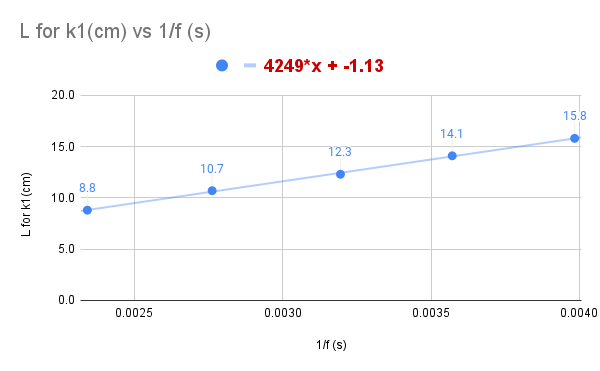
\includegraphics[scale=0.55]{L_K1.png}
	\caption{نمودار تغییرات مکان اولین گره‌ی صوتی به ازای فرکانس های مختلف}
	\label{first}
\end{figure}


\begin{figure}[h!]
	\centering
	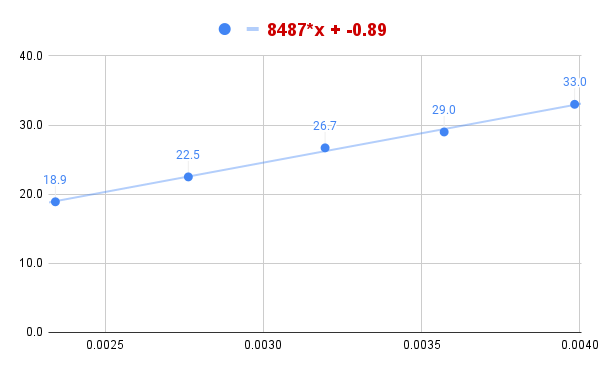
\includegraphics[scale=0.55]{L_K2.png}
	\caption{نمودار تغییرات مکان دومین گره‌ی صوتی به ازای فرکانس های مختلف}
	\label{Seconde}
\end{figure}

دمای آزمایشگاه درهنگام آزمایش برابر با 27 درجه‌ی سلسیوس گزارش شده است. مقادیر را جایگذاری می‌کنیم:
\begin{center}
$v = 141.56 + 0.61*27 \implies v = 158.03 m/s$
\end{center}

عدد بدست آمده کمتر از نصف عدد انتظاری یعنی 331 متر برثانیه می‌باشد. با اینحال بنده اعداد ناشی از گروه‌های دیگر را نیز بررسی  کردم و سرعت صوت درمقیاس و اندازه‌ی مشابه با اعداد بنده گزارش شده بودند. بنابرین محتمل است که خطای گزارش شده ناشی از خطای‌آزمایشگر و دستگاه‌های آزمایش باشد.




\section{پرسش‌ها}

1. سرعت صوت به دمای محیط و چگالی ماده‌ی داخل محیط بستگی دارد. \\
2. در این آزمایش از نوسان‌سازی استفاده کردیم که به طور دقیق توان ایجاد فرکانس های مدنظر را نداشت. و با تقریب می‌توانستیم به فرکانس مدنظر دست پیدا کنیم. از طرفی هرچقدر هم نوسان ساز دقیق کار کند، بلندگوی نصب شده برای ایجاد تپ های صوتی با دقت بالا طراحی نشده است. بنابرین می‌تواند این مساله باعث خطا باشد. \\
3. بله ولی ضرایب داخل فرمول دچار تغییر خواهند شد.



\end{document}